\documentclass[11pt]{amsart}
\usepackage{geometry}                % See geometry.pdf to learn the layout options. There are lots.
\geometry{letterpaper}                   % ... or a4paper or a5paper or ... 
%\geometry{landscape}                % Activate for for rotated page geometry
%\usepackage[parfill]{parskip}    % Activate to begin paragraphs with an empty line rather than an indent
\usepackage{graphicx}

\title{Noise Estimates for QRT}
\author{Adam Anderson}
%\date{}                                           % Activate to display a given date or no date

\begin{document}
\maketitle
\section{Overview}
In this note we estimate the noise sources in the QRT and introduce some basic notions that are necessary for performing these calculations. Much of this discussion rehashes some fairly basic concepts that can be found in a good introductory book on radio astronomy, but we included it here for completeness.


\section{Preliminaries}
All radio telescopes at their most basic level are basically an antenna which converts the electromagnetic radiation of the incoming radio waves into a small voltage that somehow gets amplified and digitized as a sequence of numbers by a computer. This sequence of numbers---the data---hopefully is related to the total power of the incoming radiation that we want to measure with some extra noise added along the way by the electronics (more on this later). In this note, we are concerned with a few questions:
\begin{enumerate}
\item {\bf What physical sources will produce that voltage at the antenna?:} If the telescope points at some radio source, like the sun, obviously that will contribute. But there is also radio emission from the ground, atmosphere, and manmade sources, which we need to account for.
\item {\bf How much power is produced in the antenna by potential sources compared with these backgrounds?:} The ``signal-to-background'' ratio clearly affects whether a potential source is detectable, and also how much data is needed to detect it.
\item {\bf How much noise is introduced by the electronics and how do we compare this with the power in the antenna?:} All electronics produce some noise, and we need to compare the power from these noise sources to the power at the antenna from the sky.
\end{enumerate}

\subsection{Noise Temperature}
All objects at finite temperatures are absorbing and emitting thermal radiation. A \emph{blackbody} is an idealized object which absorbs all incident radiation so that any radiation that it emits is due to its temperature. Although a perfect blackbody doesn't exist, it is a useful concept because many objects can be reasonably approximated as blackbodies. Blackbodies emit radiation that has the following \emph{Planck} law power spectrum
\begin{equation}\label{eqn:blackbody}
B_\nu(T) = \frac{2h\nu^3}{c^2} \frac{1}{e^{h \nu/k_B T} - 1},
\end{equation}
with units of power per area of the blackbody per unit solid angle per frequency, and where $\nu$ is the frequency of interest and $T$ is the temperature of the blackbody.

This is all interesting, but it's really more complicated than we need. Objects near a radio telescope are likely to be at a temperature of about 300~K on a spring day in Chicago, but we are interested detecting radiation that has a frequency of about 1~GHz. If we explicitly calculate the exponent in the denominator in (\ref{eqn:blackbody}), it turns out to be very small
\begin{equation}
\frac{h\nu}{k_B T} = \frac{(6.626 \times 10^{-34}~\textrm{J}\cdot\textrm{s})(10^9~\textrm{s}^{-1})}{(1.381 \times 10^{-23}~\textrm{J} \cdot \textrm{K}^{-1})(300~\textrm{K})} \sim 10^{-4} \ll 1
\end{equation}
This means that we can Taylor expand the exponential in the Planck formula in the small parameter $\hbar \omega/k_B T$, to obtain the \emph{Rayleigh-Jeans} formula
\begin{equation}\label{eqn:RayleighJeans}
B_\nu(T) \simeq \frac{h\nu^3}{c^2} \frac{1}{1 + h \nu/k_B T - 1} = \frac{2k_B T\nu^2}{c^2}.
\end{equation}
What is clear from this expression is that the noise at a given frequency is just linearly dependent on the temperature of the source.

To calculate the power from an approximate blackbody near a radio telescope, we could just plug a temperature into equation (\ref{eqn:RayleighJeans}), calculate the power, and add it to the other sources of power. But astronomers add an extra twist that is simultaneously confusing and useful. Rather than comparing the different sources of power at the antenna in terms of an SI unit like watts, radio astronomers convert a power $P$ into the temperature $T$ that a blackbody would have in order to radiate a power $P$. This means that instead of saying, ``the sky produces 10 \emph{milliwatts} of power in my telescope," the radio astronomer will say, ``the sky noise is 10 \emph{Kelvin}". This ``equivalent" temperature is called the \emph{antenna temperature}, and it is the units in which we will do all our noise estimates. Why is this madness useful? Well, it makes it trivial to compare powers to approximate blackbody sources. Since the ground, for example, is at 300~K, its noise temperature is 300~K, and we can compare other noise temperatures to it with ease.

\subsection{From Sources to Antenna Signal}
Suppose we point our telescope at some blackbody. What noise temperature will we see in the antenna? A realistic antenna is not equally sensitive to radiation from any direction\footnote{One helpful piece of jargon: an antenna that \emph{is} equally sensitive to radiation from all directions is called \emph{isotropic}.}. Instead, we need to compute a quantity called the \emph{radiation pattern}, which basically tells us, as a function of direction, how sensitive we are to incoming radiation, and then integrate this in the direction of the blackbody source.

The radiation pattern is a function $g(\theta, \phi)$ of direction\footnote{Hence we can write it as a function in terms of spherical polar coordinates}, and it normalized so that it has a maximum value of 1. Suppose our source occupies some finite angle in the sky and has a temperature as a function of direction given by $T(\theta, \phi)$. Then antenna temperature of the source is just the integral
\begin{equation}\label{eqn:antennanoise}
T_a = \frac{1}{\Delta \Omega} \int d\Omega~g(\theta, \phi) T(\theta, \phi),
\end{equation}
where the normalization factor is just the integral of the radiation pattern
\begin{equation}
\Delta \Omega = \int d\Omega~g(\theta, \phi).
\end{equation}

%\subsection{Antenna-Referred Noise}
%Assuming we can simulate the radiation pattern of our antenna, the previous two sections give everything needed for crude estimates and comparisons of signals in an antenna. But how do we compare the antenna noise to noise produced by electronics such as amplifiers, which are located \emph{after} the antenna? The answer is similar to what we did above when we defined antenna temperature: ``refer" the noise to the antenna by calculating what antenna noise temperature would give rise to the electronics noise we see later on in the circuit.


\section{Noise Sources}
\subsection{Ground Noise}
Let's assume for a minute that we have simulated the radiation pattern $g(\theta, \phi)$ of our antenna and feedhorn. As an example of this, I simulated the version 0 design of ``dipole in coffee can", whose geometry is shown in Figure~\ref{fig:cangeometry} and whose normalized gain is shown in Figure~\ref{fig:normalizedgain}.

\begin{figure}
\begin{center}
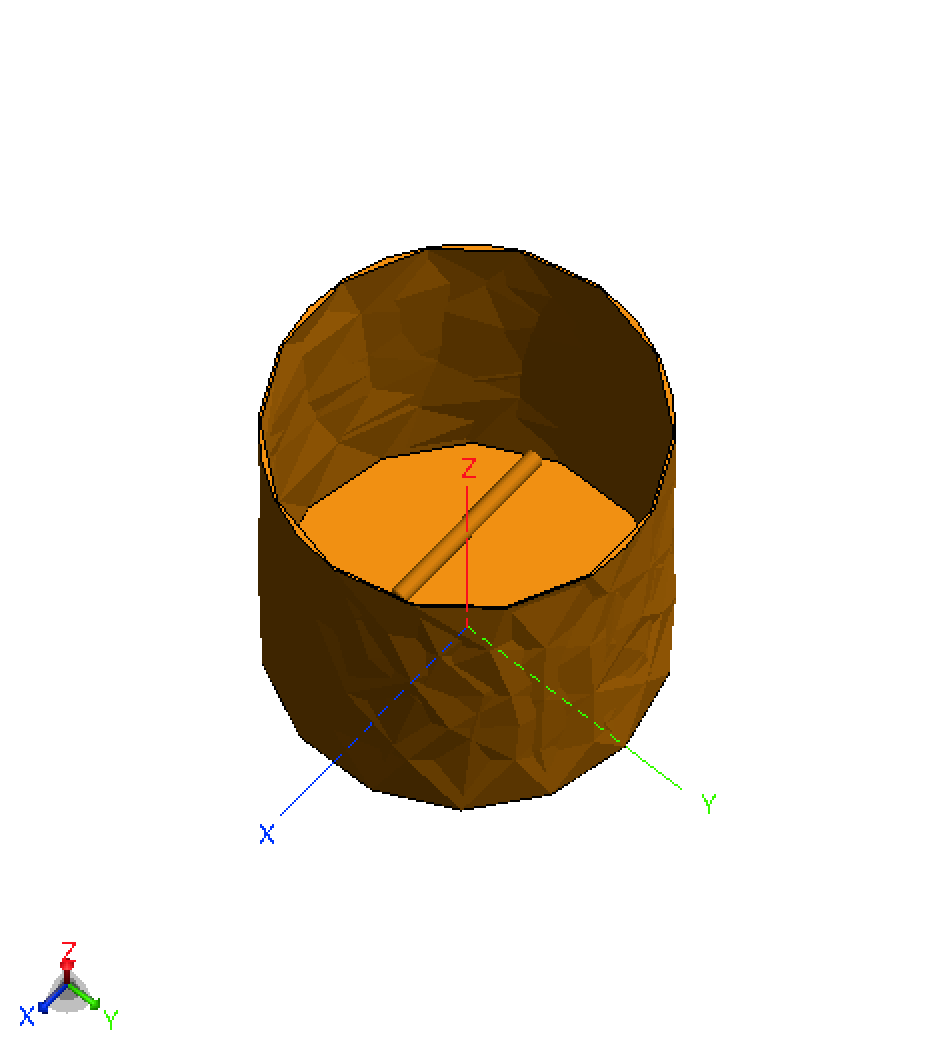
\includegraphics[width=0.5\textwidth]{figures/feedgeometry.png}
\end{center}
\caption{Geometry of antenna and feed simulated with FEKOlite.\label{fig:cangeometry}}
\end{figure}

\begin{figure}
\begin{center}
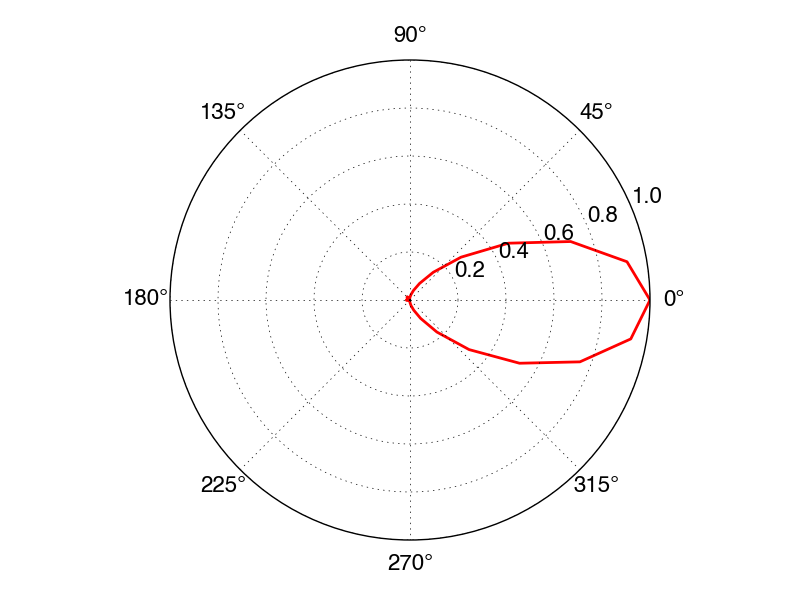
\includegraphics[width=0.5\textwidth]{figures/coffeecan_normalizedgain.png}
\end{center}
\caption{Normalized antenna gain for antenna + feed geometry simulated with FEKOlite. This shows the gain in a slice of along the $x$-axis, with $\phi=0$ and $\phi=\pi$, and the plotted angular variable representing the polar angle $\theta$ in spherical coordinates. \label{fig:normalizedgain}}
\end{figure}

With the normalized gain in hand from FEKO, we simply need to do the integral in equation (\ref{eqn:antennanoise}). Unfortunately our beam doesn't have a simple analytic form since we got it from a simulation, so we are relegated to doing the integral numerically if we want accurate results. With a little effort involving Python and interpolating functions, this can be done, and the answer is
\begin{equation}
T_{ground} = 9.4~\textrm{K}.
\end{equation}

A few comments to bear in mind:
\begin{itemize}
\item Due to the limitations of FEKOlite, I was only able to simulate the feed and antenna. We also need to include the dish. This would be a great project for someone, such as Lucas, who has access to the full version of FEKO.
\item Does this seem reasonable? You might object that this noise seems outlandishly too high given the beam shape in Figure~\ref{fig:normalizedgain}. There are larger sidelobes pointing down toward the ground in other ``slices'' besides the slice through the $x$-axis. My current understanding is that this accounts for the non-negligible ground temperature.
\end{itemize}

\subsection{Atmospheric Noise}
A variety of atmospheric processes can produce detectable power. This power is both a function of frequency and zenith angle: obviously if we are looking at angles closer to the horizon, the column of atmosphere that we are looking through is larger than when we are looking directly up. Around 1~GHz, there is a  large range of noise temperatures that depend on conditions and angle, but the temperature is roughly bracketed by
\begin{equation}
T_{atm} \sim 10-100~\textrm{K}.
\end{equation}

\begin{figure}
\begin{center}
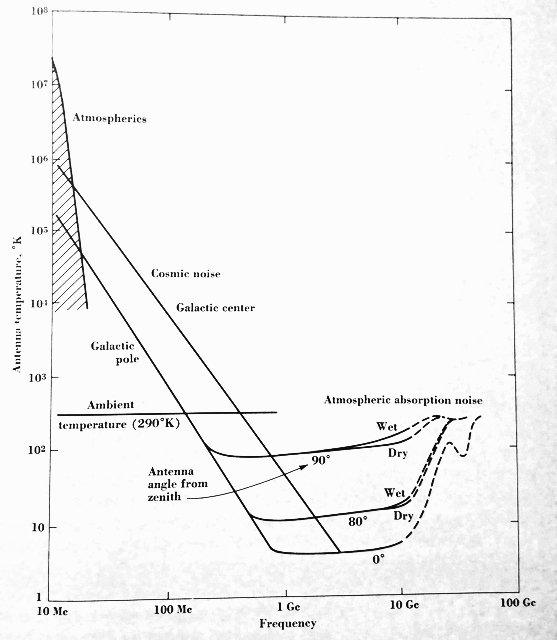
\includegraphics[width=0.7\textwidth]{figures/atmosphericnoise.png}
\end{center}
\caption{Atmospheric sky noise temperature as a function of frequency and zenith angle, from \emph{Radio Astronomy} by Kraus.\label{fig:atmosphericnoise}}
\end{figure}

\subsection{Amplifier Noise}
The preamplifier which we connect to the antenna introduces some electronics noise. We can characterize the amplifier noise by a quantity called the \emph{noise figure}
\begin{equation}
F = 1 + \frac{T_e}{T_0 = 290~\textrm{K}},
\end{equation}
where $T_e$ is the noise temperature of the amplifier. Physically, this is telling us: what is the noise power introduced by the device, relative to the power that would be produced by a blackbody at the antenna with a temperature of 290~K, and it is typically measured in dB. For our MiniSystems ZX60-P33ULN+ amplifier, the noise figure is about 0.4~dB around 1~GHz. This means that the noise temperature introduced by the amplifier is
\begin{equation}
T_e = (290~\textrm{K}) (1 - 10^{0.4 / 10}) = 290~\textrm{K} \times 0.096 = 27.8~\textrm{K}.
\end{equation}

This noise is introduced at the amplifier, but so far we are comparing our noises at the antenna. For now let's assume perfect transmission, so that we can directly compare this ground and atmospheric noise powers. In reality, we will need to account for losses between the antenna and the amplifier because the antenna is almost certainly not perfectly impedance-matched to our 50~$\Omega$ MiniSystems ZX60-P33ULN+ amplifier. These noise losses are potentially a very large contribution to the noise if the impedance is not matched well.

\section{Summary}
We have identified a few sources of power from our radio telescope setup: ground pickup, atmospheric noise, and electronics noise. A very crude estimate of the noise temperatures is
\begin{equation}
T = T_{ground} + T_{atm} + T_{e} = 9.8~\textrm{K} + 10~\textrm{K} + 27.8~\textrm{K}.
\end{equation}
By contrast, the sun has a temperature of order $10^4$~K. Although the antenna temperature depends strongly on the shape of the beam, it should be easily detectable as a first diagnostic.

\end{document}